\section{Sweet spots from higher-order corrections}
\label{higher-order app}

\begin{figure}
    \centering
    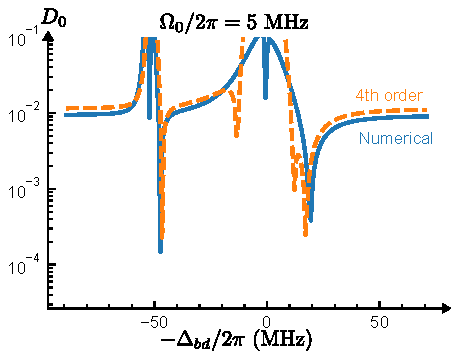
\includegraphics[width=0.9\linewidth]{Appendix/higher_order.pdf}
    \caption{Susceptibility $D_0$ including higher-order corrections in the Schrieffer--Wolff expansion. An additional sweet spot appears near $-\Delta_{bd}\simeq K/2$, arising from hybridization between $|g\rangle$ and $|f\rangle$ states}
    \label{fig:higher-order}
\end{figure}

Higher-order, drive-induced terms in the Schrieffer--Wolff expansion modify the cavity susceptibility and can generate additional flux sweet spots.
To illustrate this effect, we consider the vacuum transition frequency \(\widetilde{\omega}_{c,0\rightarrow 1}\).
Retaining terms up to fourth order yields the drive-induced correction
\begin{equation}
\begin{aligned}
&\widetilde{\omega}_{c,0\rightarrow 1}
=\overline{\omega}_c +
\frac{\Omega_0^2}{-\Delta_{bd}-\chi}
+\frac{\Omega_0^2}{\Delta_{bd}}
-\frac{\Omega_0^4}{(-\Delta_{bd}-\chi)^3}
 \\
&+\frac{2\Omega_0^4}{(-\Delta_{bd}-\chi)^2(-2\Delta_{bd}-K-2\chi)}-\frac{\Omega_0^4}{\Delta_{bd}^3}\\
&-\frac{2\Omega_0^4}{\Delta_{bd}^2(-2\Delta_{bd}-K)} .
\end{aligned}
\end{equation}

The resulting susceptibility \(D_0\) is shown in Fig.~\ref{fig:higher-order}.
In addition to the sweet spots predicted at leading order, an extra sweet spot appears near \(-\Delta_{bd}\simeq K/2\).

This feature originates from near-resonant hybridization between \(\ket{g,m}\) and the higher FTT level \(\ket{f,m}\).
At this detuning, the drive couples states separated by approximately the anharmonicity \(K\), producing an additional Stark shift that alters the cancellation condition for \(D_0\).
Operation at this sweet spot may therefore be more sensitive to drive-induced decoherence channels and should be assessed accordingly.